\begin{table}[t]
    \centering
    \begin{minipage}[c]{0.48\textwidth}
        \centering
        % \begin{figular}
        \centering
        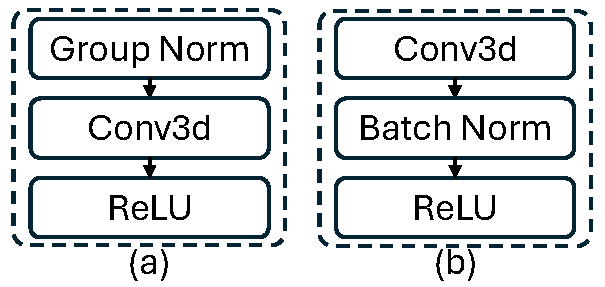
\includegraphics[width = 0.7\linewidth]{fig/CNN_block.pdf}
        \captionof{figure}{Illustration of two variants of CNN blocks in HRNet. (a) Ours (Radar-Doppler). (b) Traditional Block (RGB-Vision).}
        \label{fig:block}
        % \end{figular}

    \end{minipage}
    \hspace{0.02\textwidth}
    \begin{minipage}[c]{0.48\textwidth}
        \centering
        % \vspace{-24pt}
        \caption{
        Comparison of common 4D radar tensor-based HPE head and ours.
        }
        % \label{tab4}
        \resizebox{0.9\linewidth}{!}{
        \begin{tabular}{l|cc}
        \toprule
        HPE Head           & MPJPE~(cm) & Abs-MPJPE~(cm) \\ \midrule
                   RF-Pose3D~\cite{zhao2018rf}                  &                              15.52              &               18.08                                 \\ 
        Ours                       &             10.24                               &                     17.63                          \\ 
        \bottomrule
        \end{tabular}
        }
        \label{tab:head}
    \end{minipage}
\end{table}